\section{Queueing networks}

\subsection*{1.}

\subsubsection*{a)}

e = empty, s = in service, b = blocked

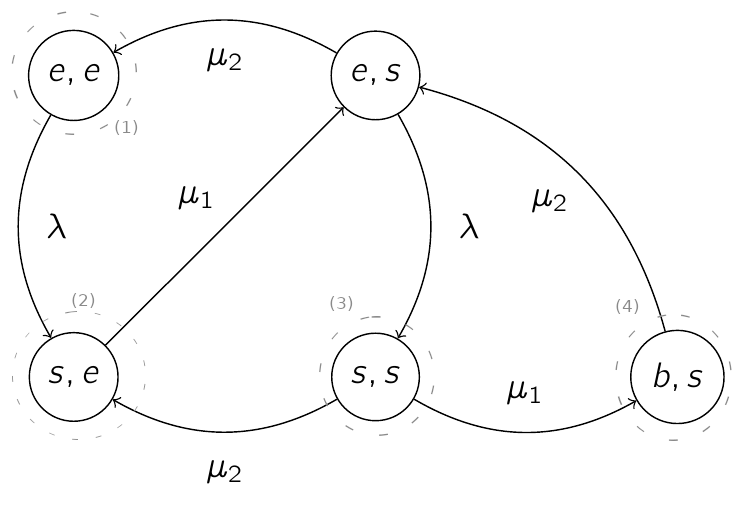
\includegraphics[width=0.65\textwidth]{pics/queue_nets_1_a.png}

\subsubsection*{b)}

stationary distribution $\rightarrow$ global balance equations:
\begin{align*}
\left(1\right)\lambda \cdot p\left(e,e\right)&=\mu _{2}\cdot p\left(e,s\right)\\
\left(2\right)\lambda \cdot p\left(e,e\right)+\mu _{2}\cdot p\left(s,s\right)&=\mu _{1}\cdot p\left(s,e\right)\\
\left(3\right)\lambda \cdot p\left(e,s\right)&=\left(\mu _{2}+\mu _{1}\right)\cdot p\left(s,s\right)\\
\left(4\right)\mu _{1}\cdot p\left(s,s\right)&=\mu _{2}\cdot p\left(b,s\right)
\end{align*}
normalization condition: $1=p\left(e,e\right)+p\left(s,e\right)+p\left(e,s\right)+p\left(s,s\right)+p\left(b,s\right)$
\begin{align*}
\cdots
\end{align*}
\begin{align*}
p ( e , e ) &= \frac { \mu _ { 1 } \mu _ { 2 } ^ { 2 } \left( \mu _ { 1 } + \mu _ { 2 } \right) } { \mu _ { 1 } \mu _ { 2 } ^ { 2 } \left( \mu _ { 1 } + \mu _ { 2 } \right) + \lambda \mu _ { 2 } \left( \mu _ { 1 } + \mu _ { 2 } \right) ^ { 2 } + \lambda ^ { 2 } \left( \mu _ { 1 } ^ { 2 } + \mu _ { 1 } \mu _ { 2 } + \mu _ { 2 } ^ { 2 } \right) }\\
p ( e , s ) &= \frac { \lambda \mu _ { 1 } \mu _ { 2 } \left( \mu _ { 1 } + \mu _ { 2 } \right) } { \mu _ { 1 } \mu _ { 2 } ^ { 2 } \left( \mu _ { 1 } + \mu _ { 2 } \right) + \lambda \mu _ { 2 } \left( \mu _ { 1 } + \mu _ { 2 } \right) ^ { 2 } + \lambda ^ { 2 } \left( \mu _ { 1 } ^ { 2 } + \mu _ { 1 } \mu _ { 2 } + \mu _ { 2 } ^ { 2 } \right) }\\
p ( s , s ) &= \frac { \lambda ^ { 2 } \mu _ { 1 } \mu _ { 2 } } { \mu _ { 1 } \mu _ { 2 } ^ { 2 } \left( \mu _ { 1 } + \mu _ { 2 } \right) + \lambda \mu _ { 2 } \left( \mu _ { 1 } + \mu _ { 2 } \right) ^ { 2 } + \lambda ^ { 2 } \left( \mu _ { 1 } ^ { 2 } + \mu _ { 1 } \mu _ { 2 } + \mu _ { 2 } ^ { 2 } \right) }\\
p ( s , e ) &= \frac { \lambda \mu _ { 2 } ^ { 2 } \left( \lambda + \mu _ { 1 } + \mu _ { 2 } \right) } { \mu _ { 1 } \mu _ { 2 } ^ { 2 } \left( \mu _ { 1 } + \mu _ { 2 } \right) + \lambda \mu _ { 2 } \left( \mu _ { 1 } + \mu _ { 2 } \right) ^ { 2 } + \lambda ^ { 2 } \left( \mu _ { 1 } ^ { 2 } + \mu _ { 1 } \mu _ { 2 } + \mu _ { 2 } ^ { 2 } \right) }\\
p ( b , s ) &= \frac { \lambda ^ { 2 } \mu _ { 1 } ^ { 2 } } { \mu _ { 1 } \mu _ { 2 } ^ { 2 } \left( \mu _ { 1 } + \mu _ { 2 } \right) + \lambda \mu _ { 2 } \left( \mu _ { 1 } + \mu _ { 2 } \right) ^ { 2 } + \lambda ^ { 2 } \left( \mu _ { 1 } ^ { 2 } + \mu _ { 1 } \mu _ { 2 } + \mu _ { 2 } ^ { 2 } \right) }
\end{align*}

\subsubsection*{c)}

\begin{align*}
E\left[S\right]&=1\cdot \left(p\left(s,e\right)+p\left(e,s\right)\right)+2\cdot \left(p\left(s,s\right)+p\left(b,s\right)\right)+0\cdot p\left(e,e\right)\\
E\left[S\right]&=\cdots\\
E [ S ] &= \frac { \lambda \left[ \lambda \left( 2 \mu _ { 1 } ^ { 2 } + 2 \mu _ { 1 } \mu _ { 2 } + \mu _ { 2 } ^ { 2 } \right) + \mu _ { 2 } \left( \mu _ { 1 } + \mu _ { 2 } \right) ^ { 2 } \right] } { \mu _ { 1 } \mu _ { 2 } ^ { 2 } \left( \mu _ { 1 } + \mu _ { 2 } \right) + \lambda \mu _ { 2 } \left( \mu _ { 1 } + \mu _ { 2 } \right) ^ { 2 } + \lambda ^ { 2 } \left( \mu _ { 1 } ^ { 2 } + \mu _ { 1 } \mu _ { 2 } + \mu _ { 2 } ^ { 2 } \right) }
\end{align*}

\subsubsection*{d)}
$p\left(e,e\right)+p\left(e,s\right)$ = proportion of time arrival can
actually occur = when 1st node is empty(e)
\begin{align*}
\lambda _{eff}&=\lambda \cdot \left(p\left(e,e\right)+p\left(e,s\right)\right)\\
\lambda _{eff}&=\cdots\\
\lambda _ {  eff } &= \frac { \lambda \mu _ { 1 } \mu _ { 2 } \left( \lambda + \mu _ { 2 } \right) \left( \mu _ { 1 } + \mu _ { 2 } \right) } { \mu _ { 1 } \mu _ { 2 } ^ { 2 } \left( \mu _ { 1 } + \mu _ { 2 } \right) + \lambda \mu _ { 2 } \left( \mu _ { 1 } + \mu _ { 2 } \right) ^ { 2 } + \lambda ^ { 2 } \left( \mu _ { 1 } ^ { 2 } + \mu _ { 1 } \mu _ { 2 } + \mu _ { 2 } ^ { 2 } \right) }
\end{align*}

\pagebreak

\subsubsection*{e)}


\begin{align*}
p_{block} &= P[\text{admitted customer gets blocked}]
\end{align*}

blocking requires two conditions: 
\begin{itemize}
\item first server is empty on arrival and second server is serving
\item service of 1st node finishes before 2nd node
\end{itemize}

\begin{align*}
p_{block} &= P[(e,s) \text{ on arrival x 1st service finishes before 2nd } | \text{ customer is admitted }]\\
&= P[(e,s) \text{ on arrival \textbar customer is admitted} ] \cdot P[\text{1st service finishes before 2nd}]\\ 
&= \frac{p\left(e,s\right)}{p\left(e,e\right)+p\left(e,s\right)}\cdot \frac{\mu _{1}}{\mu _{1}+\mu _{2}}\\
&= \frac { \lambda \mu _ { 1 } } { \left( \lambda + \mu _ { 2 } \right) \left( \mu _ { 1 } + \mu _ { 2 } \right) }
\end{align*}

\subsubsection*{f)}

\begin{align*}
E\left[D\right]&=\frac{E\left[S\right]}{\lambda _{eff}}&& \text{-  little's law -}\\
&=\ldots \\
&=\frac{\left(\lambda +\mu _{2}\right)\left(\mu _{1}+\mu _{2}\right)^{2}+\lambda \cdot \left(\mu _{1}\right)^{2}}{\mu _{1}\cdot \mu _{2}\cdot \left(\lambda +\mu _{2}\right)\left(\mu _{1}+\mu _{2}\right)}\\
&=\frac{1}{\mu _{1}}\cdot \mu _{2}+p_{block}\cdot \frac{1}{\mu _{2}}
\end{align*}


\subsection*{2.}

we solve without allowing use of reversibility property otherwise Burke's theorem
would immediately lead to the solution.

\begin{itemize}
\item  $T$: distribution of time between departures
\item  $s_{1}$: system content just before departure
\item  $s_{1}-1$: system content just after departure
\item  $d_{0}=Pr\left[s_{1}-1=0\right]$
\item  $1-d_{0}=Pr\left[s_{1}-1> 0\right]$
\end{itemize}

\begin{itemize}
\item  (i) $s-1> 0\rightarrow T\sim Exp \left(|\mu\right)$
\item  (ii) $s-1=0\rightarrow T\approx Exp \left(|\lambda\right)+Exp \left(|\mu\right)$
\end{itemize}

\begin{align*}
T^{\ast}\left(s\right)&=E\left[e^{{-sT}}\right]=E\left[E\left[e^{{-sT}}|s_{1}-1\right]\right]\\
&=E\left[e^{{-sT}}|s_{1}-1=0\right]\cdot d_{0}+E\left[e^{{-sT}}|s_{1}-1> 0\right]\cdot \left(1-d_{0}\right)\\
&=d_{0}\cdot \frac{\lambda }{\lambda +s}\cdot \frac{\mu }{\mu +s}+\left(1-d_{0}\right)\cdot \frac{\mu }{\mu +s}
\end{align*}

We know from 3.14: system content after departure $\sim $ system content at arrival instants

through PASTA we know: $d_{0}=1-\rho ,\rho =\frac{\lambda }{\mu }$

\begin{align*}
T^{{\ast }}\left(s\right)&=\frac{\lambda }{\lambda +s}\implies T\sim Exp \left(\ldots |\lambda \right)&& \text{-  $\rightarrow$ same as with Burke -}
\end{align*}

\subsection*{3.}

\subsubsection*{a)}

Define $S_i$ as nr of customers in node $i, i=1,2$. Then $(S_1, S_2)$ is a CTMC with state space $\mathbb{N} \times \mathbb{N}$ and state transition diagram:

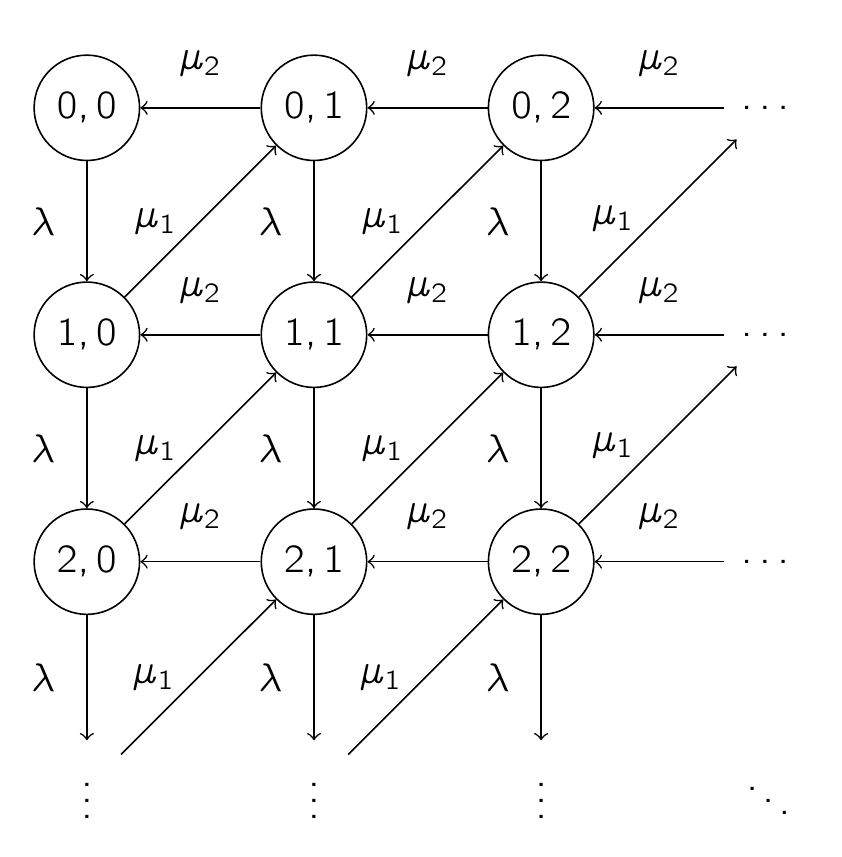
\includegraphics[width=0.65\textwidth]{pics/state_trans_que_nets_3.png}

\subsubsection*{b)}

\begin{align*}
\lambda s ( 0,0 ) &= \mu _ { 2 } s ( 0,1 )\\
\left( \lambda + \mu _ { 1 } \right) s \left( n _ { 1 } , 0 \right) &= \lambda s \left( n _ { 1 } - 1,0 \right) + \mu _ { 2 } s \left( n _ { 1 } , 1 \right)\\
\left( \lambda + \mu _ { 2 } \right) s \left( 0 , n _ { 2 } \right) &= \mu _ { 1 } s \left( 1 , n _ { 2 } - 1 \right) + \mu _ { 2 } s \left( 0 , n _ { 2 } + 1 \right)\\
\left( \lambda + \mu _ { 1 } + \mu _ { 2 } \right) s \left( n _ { 1 } , n _ { 2 } \right) &= \lambda s \left( n _ { 1 } - 1 , n _ { 2 } \right) + \mu _ { 1 } s \left( n _ { 1 } + 1 , n _ { 2 } - 1 \right) + \mu _ { 2 } s \left( n _ { 1 } , n _ { 2 } + 1 \right)
\end{align*}

\subsection*{4.}

\textbf{used formulas}

\begin{itemize}
\item  M/M/1 with arrival rate $\lambda $, service rate $\mu $
\item  $Pr\left[s=n\right]=\left(1-\rho \right)\rho ^{n}$ with $\rho =\frac{\lambda }{\mu }$, $n=0,1,2\ldots$ 
\item $E\left[S\right]=\frac{\lambda }{\mu -\lambda }=\frac{\rho }{\rho -1}$
\end{itemize}

\textbf{solution}

\subsubsection*{ a) }

stability condition for Jackson network: $\lambda \le \mu $
$\implies $ for our network: $2\cdot \lambda < \mu _{1}+\mu _{2}$  $\implies $ $\lambda _{1}=\lambda _{2}=\lambda $
$\implies $ Burke's theorem

\subsubsection*{ b) }

$E\left[D\right]=\frac{E\left[S\right]}{\lambda }$ little's law

we have a feedforward network:
\begin{align*}
E\left[S\right]&=E\left[S_{1}+S_{2}\right]\\
&=\sum _{{n_{1},n_{2}}}\left(n_{1}+n_{2}\right)\cdot Pr\left[S_{1}=n_{1},S_{2}=n_{2}\right]\\
&=\sum _{{n_{1},n_{2}}}\left(n_{1}+n_{2}\right)\cdot Pr\left[S_{1}=n_{1}\right]\cdot Pr\left[S_{2}=n_{2}\right]\\
&=E\left[S_{1}\right]+E\left[S_{2}\right]&& \text{-  because Jackson Network -}\\
&=\frac{\lambda }{\mu _{1}-\lambda }+\frac{\lambda }{\mu _{2}-\lambda }\\
&=\frac{\lambda }{\mu _{1}-\lambda }+\frac{\lambda }{\left(\mu -\mu _{1}\right)-\lambda }
\end{align*}

We minimize E[S], through Little's law this results in a minimal E[D]:

\begin{align*}
\frac{d}{d\mu _{1}}E\left[S\right]&=\frac{d}{d\mu _{1}}\left[\frac{\lambda }{\lambda -\mu _{1}}+\frac{\lambda }{\mu -\mu _{1}-\lambda }\right]=0\\
\frac{d}{d\mu _{1}}E\left[D\right]&=\frac{d}{d\mu _{1}}\left[\frac{\lambda }{\lambda -\mu _{1}}+\frac{\lambda }{\mu -\mu _{1}-\lambda }\right]=0\\
\Leftrightarrow \mu _{1}&=\frac{\mu }{2}
\end{align*}
\begin{align*}
\mu _{{1opt}}&=\frac{\mu }{2} && \mu_{1opt} \text{ in } ] \lambda, \mu - \lambda[\\ 
\mu _{{2opt}}&=\mu -\frac{\mu }{2}=\frac{\mu }{2}
\end{align*}
stability condition: $\lambda < \mu _{1}$

\subsubsection*{c)}

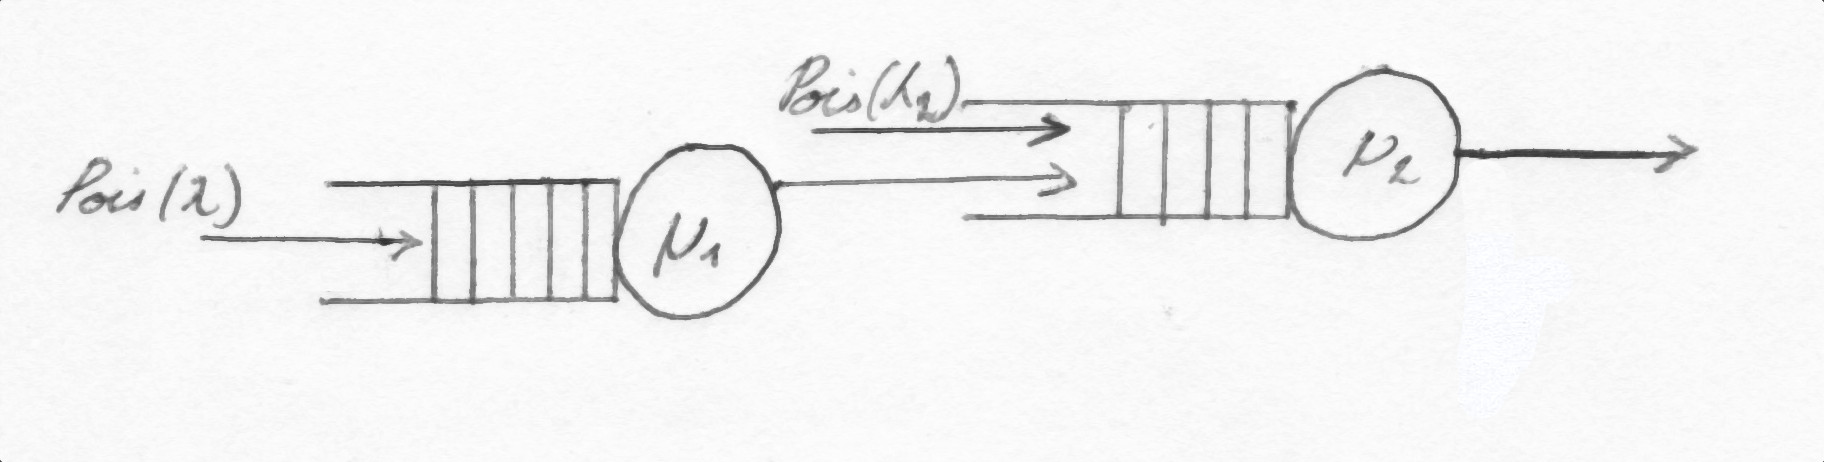
\includegraphics[width=0.75\textwidth]{pics/Ex09_jackson_net_4c.jpg}

\begin{align*}
\mu _ { 1 } = \frac { \mu - \gamma } { 2 } = \lambda + \frac { \mu - 2 \lambda - \gamma } { 2 } && \text{ and } &&
\mu _ { 2 } = \frac { \mu + \gamma } { 2 } = \lambda + \gamma + \frac { \mu - 2 \lambda - \gamma } { 2 }
\end{align*}

\subsubsection*{d)}

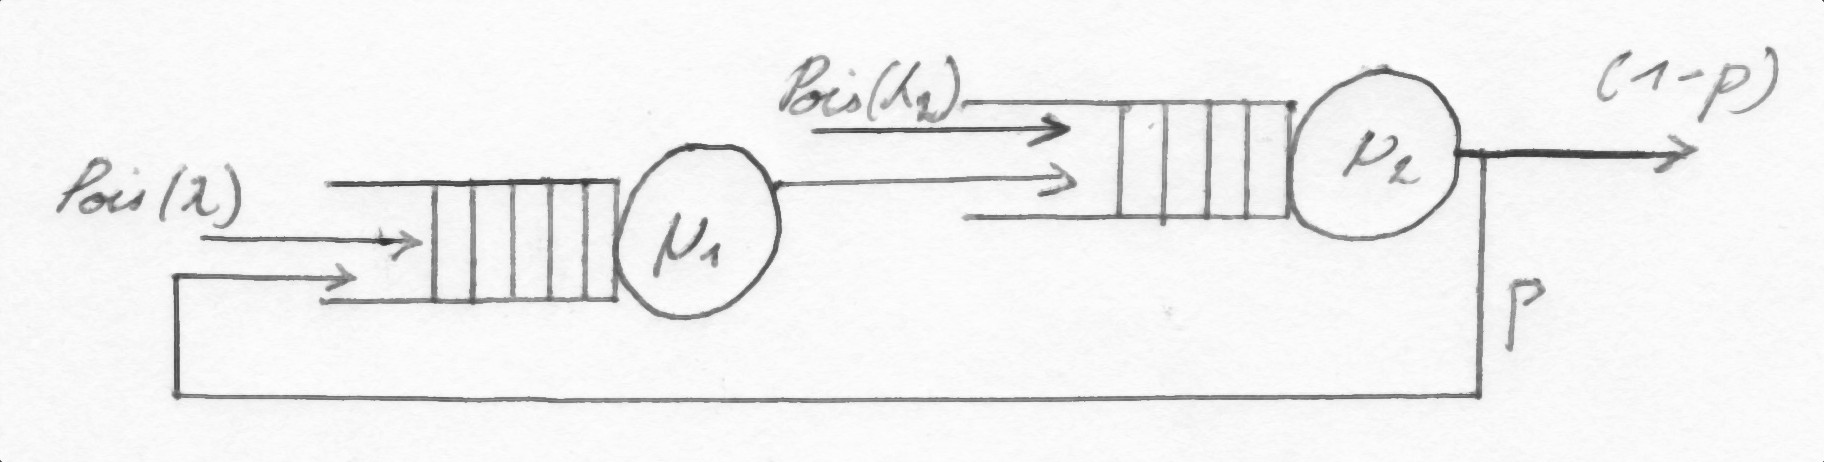
\includegraphics[width=0.75\textwidth]{pics/Ex09_jackson_net_4d.jpg}

traffic equations:
\begin{align*}
\lambda _{1}&=\lambda +p\cdot \lambda _{2}\\
\lambda _{2}&=\lambda _{1}+\gamma 
\end{align*}
\begin{align*}
\lambda _{1}&=\frac{\lambda +p\cdot \gamma }{1-p}\\
\lambda _{2}&=\frac{\lambda +\gamma }{1-p}
\end{align*}
as before we solve $\frac{dE\left[S\right]}{d\mu _{1}}=0$ for $\mu _{1} \ldots$

The constraint now becomes:

\begin{align*}
\mu > \frac { 2 \lambda + ( 1 + p ) \gamma } { 1 - p }
\end{align*}

The optimal distribution of the total service rate $\mu$ in this case is:

\begin{align*}
\mu _ { 1 } = \frac { \lambda + p \gamma } { 1 - p } + \frac { ( 1 - p ) \mu - 2 \lambda - ( 1 + p ) \gamma } { 2 ( 1 - p ) } && \text{ and } && \mu _ { 2 } = \frac { \lambda + \gamma } { 1 - p } + \frac { ( 1 - p ) \mu - 2 \lambda - ( 1 + p ) \gamma } { 2 ( 1 - p ) }
\end{align*}

\subsection*{5.}

\subsubsection*{a)}

\begin{tikzpicture}
        \node[state]             (0) {0};
        \node[state, right=of 0] (1) {1};
        \node[state, right=of 1] (2) {\ldots};
        \node[state, right=of 2] (3) {K};

        \draw[every loop]
            (0) edge[bend right, auto=right]  node {$\lambda$} (1)
            (1) edge[bend right, auto=right] node {$\mu$} (0)
            (1) edge[bend right, auto=right]  node {$\lambda$} (2)
            (2) edge[bend right, auto=right]  node {$\mu$} (1)
            (2) edge[bend right, auto=right] node {$\lambda$} (3)
            (3) edge[bend right, auto=right]  node {$\mu$} (2)
            ;
\end{tikzpicture}

Local balance equation:

\begin{align*}
\lambda s ( n ) = \mu \cdot s ( n + 1 ) && n=0,\ldots, K-1
\end{align*}

A (normalized) solution for these balance equations can be found. Therefore—see (CN: Sec-
tion 2.2, p. 6.6)—the CTMC is reversible.

\subsubsection*{b)}

Burke's theorem states that when a queue is reversible the arrival process must correspond to the departure process.
The arrival process is not poisson because customers get discarded if K customers are in the queue $\Rightarrow$ finite capacity.
